\subsection{实验目的-MSSQL攻击日志分析}
\begin{enumerate}
  \item 破解 SQL Server 2008 的 sa 密码
  \item 抓取破解过程中的数据包并分析
  \item 查看并分析 SQL Server 日志文件
\end{enumerate}
%
\subsection{实验原理}
TCP 协议与三次握手:
TCP(Transmission Control Protocol:传输控制协议) ,TCP 是主机对主机
层的传输控制协议,提供可靠的连接服务,采用三次握手确认建立一个连接。

位码即 tcp 标志位,有 6 种标示:
\begin{itemize}
  \item SYN(synchronous 建立联机)
  \item ACK(acknowledgement 确认)
  \item PSH(push 传送)
  \item FIN(finish 结束)
  \item RST(reset 重置)
  \item URG(urgent 紧急)
\end{itemize}
%
三次握手过程如下:
\begin{enumerate}
  \item 第一次握手:主机 A 发送位码为 $\texttt{SYN}=1$, 随机产生 SEQ number 的数据包到
    服务器,主机 B 由 $\texttt{SYN}=1$ 知道,A 要求建立联机;
  \item 第二次握手:主机 B 收到请求后要确认联机信息,
    向 A 发送 $\texttt{ACK number}=(\texttt{主机A的SEQ}+1),\texttt{SYN}=1,\texttt{ACK}=1$,
    随机产生 SEQ number 的包;
  \item 第三次握手:主机 A 收到后检查 ACK number 是否正确,
    即第一次发送的 $\texttt{SEQ number}+1$,
    以及位码 ack 是否为 1,若正确,
    主机 A 会再发送 $\texttt{ACK number}=(\texttt{主机B的SEQ}+1),\texttt{ACK}=1$,
    主机 B 收到后确认 SEQ 值与 $\texttt{ACK}=1$ 则连接建立成功。
\end{enumerate}
完成三次握手,主机 A 与主机 B 开始传送数据。
%
\subsection{实验环境}
\begin{itemize}
  \item Kali Linux:192.168.1.2 hydra
  \item Windows server 2003:192.168.1.3 SQL Server 2008 R2
\end{itemize}
%
\subsection{实验步骤}
\subsubsection{破解sa密码,并用wireshark抓取破解数据包}
在 Windows server 2003 上打开 wireshark,并抓取数据包。
\begin{figure}[H]
  \begin{center}
    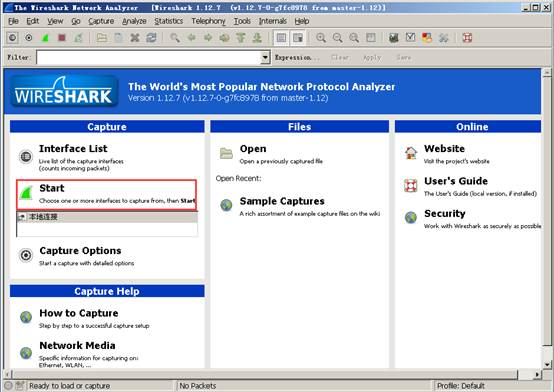
\includegraphics[width=0.40\textwidth]{2_10_1.jpeg}
  \end{center}
\end{figure}

在 Kali 上,查看用户名文件 \texttt{userlist.txt} 和
密码文件 \texttt{passlist.txt}。
\begin{figure}[H]
  \begin{center}
    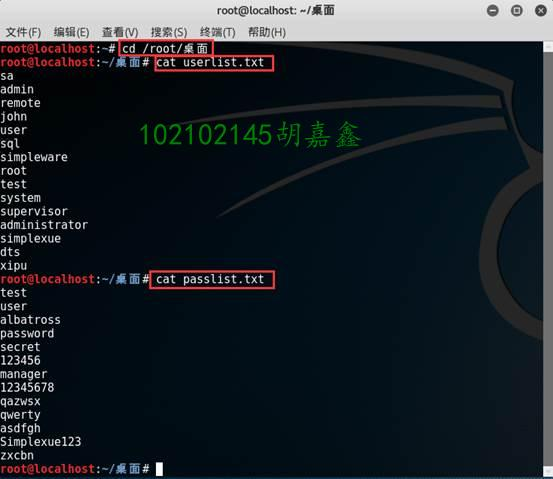
\includegraphics[width=0.40\textwidth]{2_10_2.jpeg}
  \end{center}
\end{figure}

在终端输入命令
\begin{minted}[bgcolor=bg,breaklines=true]{sh}
hydra -L userlist.txt -P passlist.txt 192.168.1.3 mssql -t 1
\end{minted}
开始破解 mssql,可以看到破解出 sa 的密码为 123456。
注意:
由于 hydra 的默认线程不是 1,为了更加便于后面数据包的分析,破解 mssql
时最好将线程数设为 1。
\begin{figure}[H]
  \begin{center}
    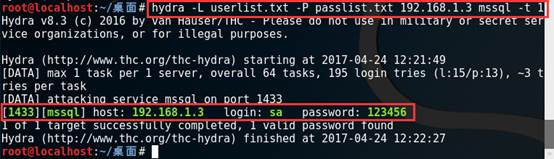
\includegraphics[width=0.40\textwidth]{2_10_3.jpeg}
  \end{center}
\end{figure}

返回 Windows server 2003,wireshark 停止抓包,
过滤端口为 1433 的数据包。
\begin{figure}[H]
  \begin{center}
    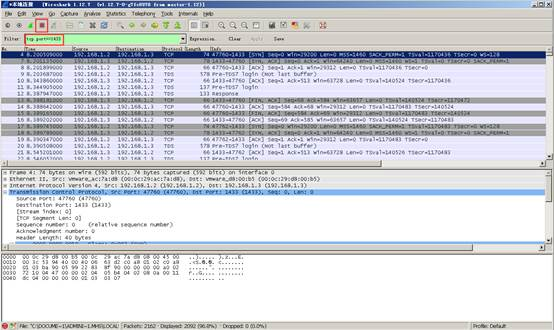
\includegraphics[width=0.40\textwidth]{2_10_4.jpeg}
  \end{center}
\end{figure}
%
\subsubsection{分析抓取的数据包,理解 mssql 破解过程}
首先查看第一个数据包,源地址为 \texttt{192.168.1.2},源端口为 \texttt{47366},
目的地址为 \texttt{192.168.1.3},目的端口为 \texttt{1433},
TCP 序号为 SYN,且置为 1,
表示客户端 \texttt{192.168.1.2} 向服务器 \texttt{192.168.1.3} 发送了一个连接请求报文。
\begin{figure}[H]
  \begin{center}
    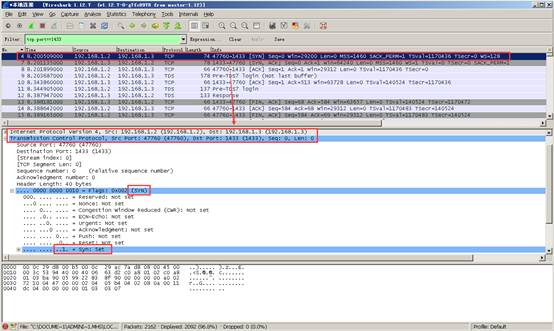
\includegraphics[width=0.40\textwidth]{2_10_5.jpeg}
  \end{center}
\end{figure}

再查看第二个数据包,\texttt{192.168.1.3} 收到请求后确认联机信息,
向 \texttt{192.168.1.2} 发送数据包,SYN 置为 1,ACK 也置为 1。
\begin{figure}[H]
  \begin{center}
    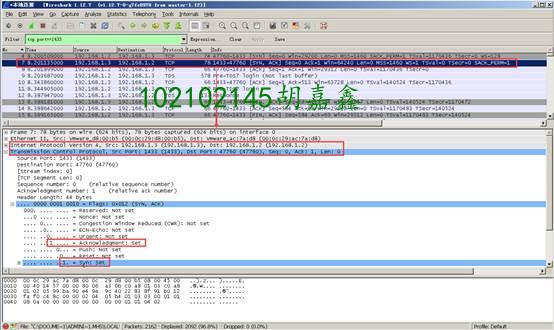
\includegraphics[width=0.40\textwidth]{2_10_6.jpeg}
  \end{center}
\end{figure}

查看第三个数据包,主机 \texttt{192.168.1.2} 收到数据包后检查无误,
向 \texttt{192.168.1.3} 发送数据包,ACK 置为 1,
至此三次握手完毕,连接建立,后面就可以开始传输数据了。
\begin{figure}[H]
  \begin{center}
    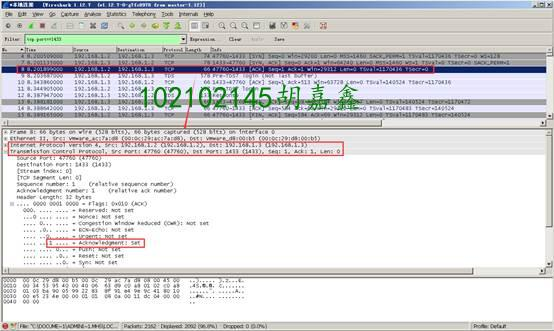
\includegraphics[width=0.40\textwidth]{2_10_7.jpeg}
  \end{center}
\end{figure}

查看第四个数据包,可以看到传输的数据,其中包括了用户名 sa 和密码 test,
表明正在破解 mssql。
\begin{figure}[H]
  \begin{center}
    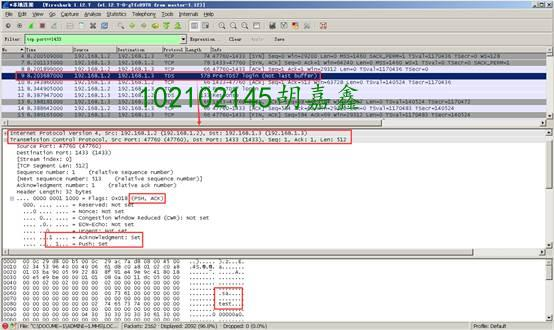
\includegraphics[width=0.40\textwidth]{2_10_8.jpeg}
  \end{center}
\end{figure}

查看 response,可以看到为 false,说明连接不成功,即用户名或者密码错
误。之后则是连接的结束过程。
\begin{figure}[H]
  \begin{center}
    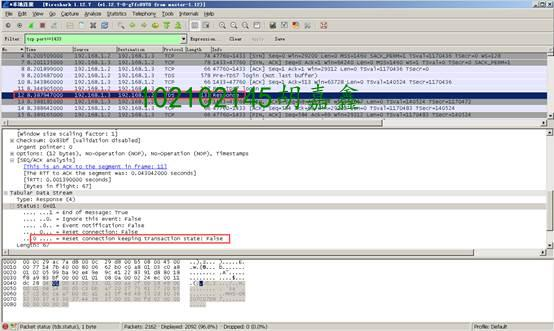
\includegraphics[width=0.40\textwidth]{2_10_9.jpeg}
  \end{center}
\end{figure}

通过分析抓取的数据包,我们可以得知,重复的过程实际上也就是 mssql 破
解的过程。
\begin{figure}[H]
  \begin{center}
    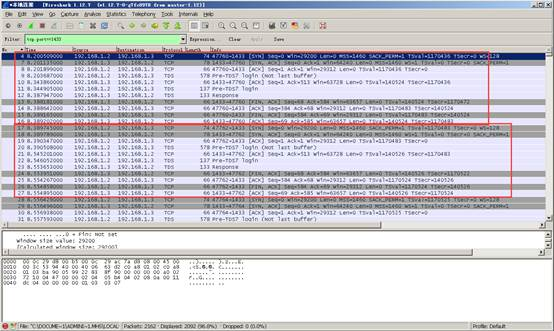
\includegraphics[width=0.40\textwidth]{2_10_10.jpeg}
  \end{center}
\end{figure}

我们找到破解出来的 sa 密码 123456 对应的数据包,并查看其 response 数
据包,发现与其它 response 数据包相比,多了一些数据,说明 sa 的密码很
有可能是 123456,实际上也的确如此。
\begin{figure}[H]
  \begin{center}
    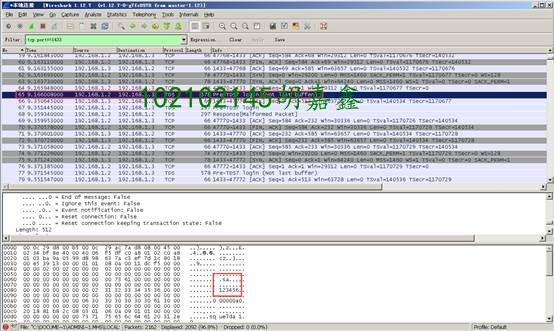
\includegraphics[width=0.40\textwidth]{2_10_11.jpeg}
  \end{center}
\end{figure}
\begin{figure}[H]
  \begin{center}
    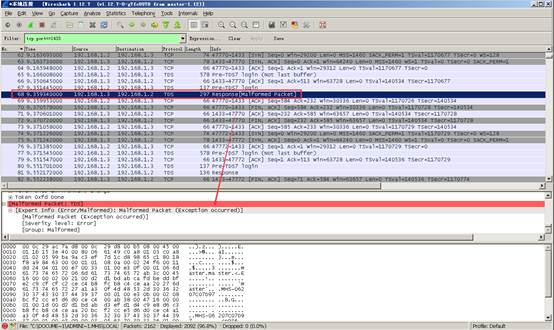
\includegraphics[width=0.40\textwidth]{2_10_12.jpeg}
  \end{center}
\end{figure}
%
\subsubsection{查看 mssql 日志}
单击``开始'' $ \rightarrow $ ``所有程序''
$ \rightarrow $ ``Microsoft SQL Server 2008 R2`` $ \rightarrow $
``SQL Server Management Studio''。
\begin{figure}[H]
  \begin{center}
    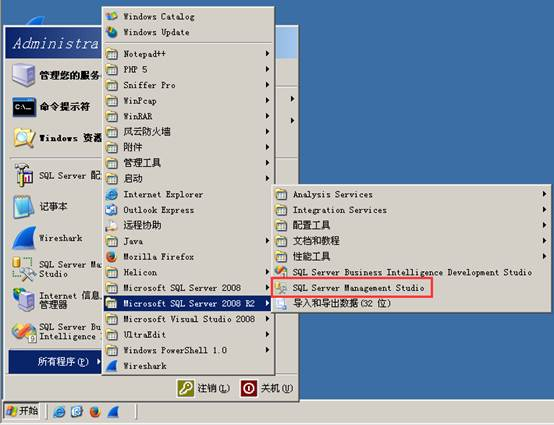
\includegraphics[width=0.40\textwidth]{2_10_13.jpeg}
  \end{center}
\end{figure}

以``Windows 身份认证''方式进行登录
(也可用前面破解出来的 \texttt{sa/123456} 进行登录,
不过登录方式要选择 SQL Server 身份认证)。
\begin{figure}[H]
  \begin{center}
    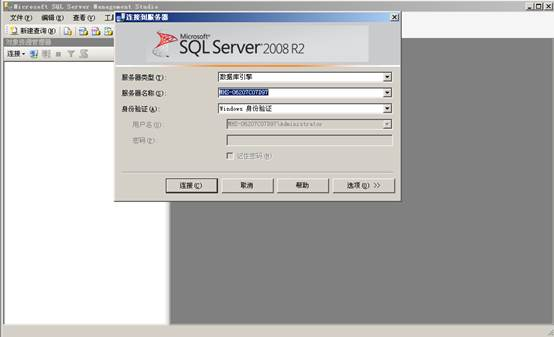
\includegraphics[width=0.40\textwidth]{2_10_14.jpeg}
  \end{center}
\end{figure}

展开``管理'' $ \rightarrow $ ``SQL Server 日志'',双击当前日志。
\begin{figure}[H]
  \begin{center}
    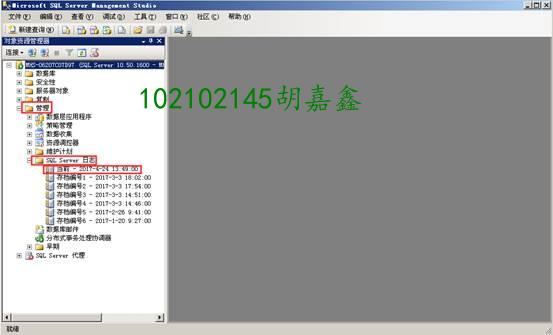
\includegraphics[width=0.40\textwidth]{2_10_15.jpeg}
  \end{center}
\end{figure}

在打开的日志文件查看器中查看到的 SQL Server 日志信息中,可以看到前
面破解过程中尝试登录的情况,例如以 xipu 用户名进行登录时,提示``找
不到与所提供的名称相匹配的登录名'',说明登录名中没有 xipu。其中,前
两条日志记录是使用 Windows 身份认证进行登录的信息。看到这么多短时间
内登录失败的日志信息,我们就可以得知数据库遭受了攻击,需要采取一定
的手段进行防御。
\begin{figure}[H]
  \begin{center}
    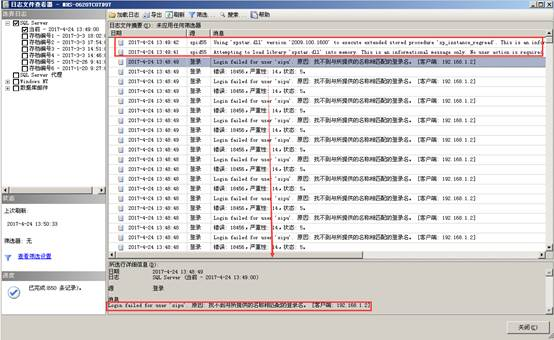
\includegraphics[width=0.40\textwidth]{2_10_16.jpeg}
  \end{center}
\end{figure}

使用 sa 尝试进行登录时,提示``密码与所提供的登录名不匹配'',说明 sa
是一个登录名。在使用 sa 破解的过程中,有两条信息与使用 Windows 身份
认证进行登录时的日志信息很相似,我们可以猜测该记录对应的 sa 密码是
正确的,实际上也的确如此。
\begin{figure}[H]
  \begin{center}
    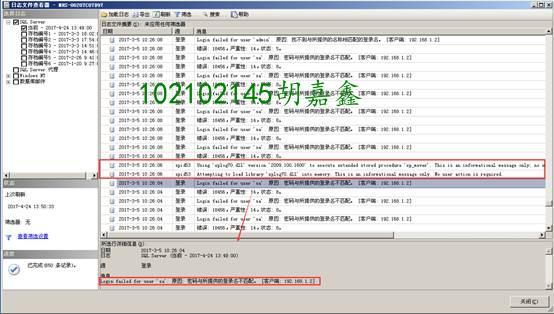
\includegraphics[width=0.40\textwidth]{2_10_17.jpeg}
  \end{center}
\end{figure}
